\documentclass[12pt,a4paper]{article}

\usepackage{amssymb}
\usepackage{amsmath}
%\usepackage{ngerman}
\usepackage[latin1]{inputenc}
\usepackage[T1]{fontenc}
\usepackage{microtype}
\usepackage{fixltx2e}
\usepackage{graphicx}

\usepackage[nosepfour]{numprint}
\usepackage{xspace}

\newcommand{\figref}[1]{Fig.~\ref{#1}}
\newcommand{\Figref}[1]{Figure~\ref{#1}}
\newcommand{\HRule}{\rule{\linewidth}{0.5mm}}

\newcommand{\bet}[1]{\begin{center}
		     \begin{tabular}{|c|c|}
		     \hline
		     \multicolumn{2}{|c|}{#1}\\
		     \hline\hline
		     input & output \\
                     \hline}
\newcommand{\eet}{\hline
		  \end{tabular}
		  \end{center}}
\newcommand{\eqnref}[1]{Eq.~\ref{#1}}

\begin{document}

%\title{GPI and MCTP, the tools for HPC}

\begin{titlepage}
 
\begin{center}
 
 
% Upper part of the page
\begin{flushright}

\includegraphics{./itwm_85mm_cmyk.eps}\\[2cm]
\end{flushright}
 
%\textsc{\LARGE University of Beer}\\[1.5cm]
 
%\textsc{\Large Project report}\\[0.5cm]
 
 
% Title
\textsc{\Large SDPA}\\[0.5cm]
\HRule \\[0.4cm]
{ \huge \bfseries object and associated operation specification }\\[0.4cm]
\HRule \\[0.4cm]
\textsc{\Large for the seismic domain}\\[0.5cm]

\vfill


\vfill
% Author and supervisor
\begin{flushright}
\begin{minipage}{0.5\textwidth}
\begin{flushleft} %\large
 \emph{Author:}\\
 Dr. Daniel Gr\"unewald\\
% Dr. Norman Ettrich\\
% Dr. Dirk Merten\\
% Dr. Martin K\"uhn
 CC HPC\\
 Fraunhofer ITWM\\
 Fraunhofer-Platz 1\\
 67663 Kaiserslautern\\ 
 {\tt daniel.gruenewald@itwm.fhg.de}
\end{flushleft}
\end{minipage}
\end{flushright}
%\begin{minipage}{0.4\textwidth}
%\begin{flushright} %\large
%\emph{Supervisor:} \\
%Dr. Mark \textsc{Brown}
%\end{flushright}
%\end{minipage}
 
% Bottom of the page
%{\large \today}
 
\end{center}
 
\end{titlepage}

%\maketitle

\newpage

\tableofcontents

\newpage

\section{Introduction}

In this report, we describe the data objects and the associated 
operations which are typically required by a seismic domain expert 
in order to describe a seismic migration work flow. 

Seismic migration is a method which is used to locate layer 
boundaries in the interior of the earth. The several migration
algorithms are applied to data samples obtained from seismic surveys. 
In these seismic surveys, sound waves are produced artificially on the 
surface. They propagate through the subsurface. If a sound wave meets a layer 
boundary, the wave is reflected and diffracted. The reflected wave propagates back to the 
surface where it is sampled with hydro- or geophones. These recorded data are the starting point
for the migration. One uses a subsurface velocity model in order to numerically propagate these 
signals back into the subsurface. The velocity model has to be provided initially and needs to be
estimated. 
At the layer boundaries, constructive interference appears and the layer boundaries become visible 
in the resulting output image. Some migration methods directly use the velocity model for the back propagation, other migration methods use them only indirectly via travel time tables. A travel time table 
holds the information how long it takes for a seismic wave to propagate from a given surface position to a given subsurface position. The travel time tables themselves are computed by ray tracing methods from the given velocity model.  

Hence, all of the seismic migration algorithms require essentially four different types of 
basic data objects in order to produce a seismic output image. One has to 
deal with spatial volumina which cover the subsurface image. The 
so called traces represent the data sampled at the surface.  
The velocity fields are an initial guess for the sound velocity 
distribution in the underground. The velocity field itself may come in three flavors. A simple one parameter scalar velocity field, a three parameter vertical transverse
isotropic (vti) velocity field and a five parameter tilted transverse isotropic (tti) velocity field. 
Then, there are also the travel time tables as the fourth object.

In addition to these atomic or elementary objects, 
also the concept of bunches or gathers respectively is important for seismic applications. An
object bunch gathers several elementary objects into a single object and helps to organize
the work flows. In summary, one needs the following objects:

\begin{itemize}
\item volumina
\begin{itemize}
\item single volume
\item volume bunch
\end{itemize}
\item traces
\begin{itemize}
\item single trace
\item trace bunch
\end{itemize}
\item travel time tables
\begin{itemize}
\item single travel time table
\item travel time table bunch
\end{itemize}
\item velocity fields
\begin{itemize}
\item single velocity field
\begin{itemize}
\item single scalar veloctiy field
\item single vti velocity field
\item single tti velocity field
\end{itemize}
\item velocity field bunch
\end{itemize}
\end{itemize}
% In principle, one has to differentiate between inter- and inner-object operations.
% Inter object operations involve two or more objects of the same kind as input and 
% have one object of the same kind as an output.
% Inner-Object operations involve only one object as an input and yield an object
% of the same kind as an output.  
The vti and tti velocity fields can be considered as being a bunch of three or five
scalar velocity fields, i.e. vti and tti velocities are only special bunch implementations of these. 
Hence, we restrict ourselves to the discussion of the simple one parameter scalar 
velocity field and the associated bunch in the following.  
In addition to these seismic specific objects, one also needs a configuration object in order to control 
the workflow.
\begin{itemize}
\item configuration
\end{itemize}
In the following sections, we first describe the operations required by the configuration
object. Then, we consider the operations which are common to
all seismic objects, both for the single objects as well as for the 
bunch objects. In section three, we discuss the operations which 
supplement the common operations for the specific objects. Then, we introduce 
a low level memory handler object and the associated operations. This is beyond 
the scope of the seismic domain. However, it helps to understand the general set up
and to complete the discussion on the seismic specific objects. 
In the last section, we use the introduced objects
and operations in order to implement an example for a 
simple seismic work flow. 

\section{flow control object}

In this section, the operations on the configuration object are described.
The configuration object is intended to manage the behavior of the 
seismic specific operations. Hence, the structure of the configuration 
object has to contain a set of parameters.
At the begining of the workflow, it needs to be read from file which is accomplished by
the following operation 
\newline
\begin{center}
\begin{tabular}{|c|c|}
\hline
\multicolumn{2}{|c|}{read config. from file}\\
\hline\hline
input & output \\
\hline
text string & configuration \\
\hline
\end{tabular}
\end{center}

\section{common seismic object operations}

In this section we present the operations which are common
to all seismic specific objects. They need to be implemented 
for each of them. We differentiate between common single object 
operations and common bunch object operations.

\subsection{common single object operations}

The structure of a single object consists essentially out of 
two parts. The first part is given by some meta data which 
uniquely characterizes the object (specific realizations of these
meta data are given in the next section). The second part corresponds
to the actual data part. Common to all single objects (obj) are the 
following operations:

\begin{itemize}
\item Copy object:
\newline
Makes a copy of the given object  
\bet{copy obj}
obj & obj \\
    & obj \\
\eet

\item Initialize object with a given value:
\newline
Initializes an object, i.e. sets all the entries 
in the data part of the object to the given value val. 
\bet{init obj}
obj        & obj\\
double val &    \\
\eet
\item Load object data from disk:
\newline
Loads the data corresponding to the object meta data from disk
\bet{load obj}
configuration & obj \\
obj & \\
\eet
\item Save object to disk:
\newline
Saves the object data to disk at the right file and at the right 
position in the file corresponding to the object meta data.
\bet{save obj}
config & obj\\
obj & \\
\eet
\item Update object on disk:
\newline
Loads the data corresponding to the object meta data from disk into
some temp space, adds the given object data
and writes the result back to disk. 
\bet{udpate obj}
config & \\
obj &    \\
\eet
\item Transpose:
\newline
Exchange the memory layout of the given object (only required
for objects with dimension $n>1$). 
The desired memory hierarchy of the $n$ directions 
is delivered by a hierarchy list. For example, in three dimensions,
the hierarchy list $\{x,z,y\}$ implies the x-direction to 
be the slowest direction and the y-direction to be the 
fastest direction.  
\bet{Transpose}
obj & obj \\
int hierachy[n] & \\
\eet
\item Add two objects ($\mathrm{obj}_3 = \mathrm{obj}_1 + \mathrm{obj}_2$):
\newline
Performs a pointwise addition of the object data 
\bet{add}
$\mathrm{obj}_1$ & $\mathrm{obj}_3$\\
$\mathrm{obj}_2$ & \\
\eet
\item Subtract two objects ($\mathrm{obj}_3 = \mathrm{obj}_1 - \mathrm{obj}_2$)
\newline
Performs a pointwise subtraction of the object data 
\bet{subtract vol}
$\mathrm{obj}_1$ & $\mathrm{obj}_3$\\
$\mathrm{obj}_2$ & \\
\eet
\item Scalar multipy an object ($\mathrm{obj}_2 = \mathrm{double} * \mathrm{obj}_1$)
\newline
Performs a pointwise multiplication of the object data with the given scalar
\bet{scal mul}
$\mathrm{obj}_1$ & $\mathrm{obj}_2$ \\
double & \\
\eet
\item Pointwise multiply two objects $\left[\mathrm{obj}_3 = \mathrm{obj}_1\cdot \mathrm{obj}_2\right]_{\mathrm{at\,each\,data\,point}}$
\newline
Performs a pointwise multiplication, i.e. each data point of the first object is multiplied 
with the correspondent data point of the second object.  
\bet{pointwise mul}
$\mathrm{obj}_1$ & $\mathrm{obj}_3$\\
$\mathrm{obj}_2$ & \\
\eet
\item Compute the $\mathrm{L}_2$ norm of the object:
\newline
The $\mathrm{L}_2$ norm of an object is given by the summing up the 
square of each data point. At the end, the square root of the result is taken. 
\bet{$\mathrm{L}_2$}
obj & double\\
\eet
\item Fourier transform obj ($\mathrm{obj}_2 = \mathrm{FFT}(\mathrm{obj}_1,\mathrm{dir})$). A flag 
represented by an integer decides whether the Fourier transform or its inverse
are computed. In the case of higher dimensional data like volumina, velocity fields or travel time tables,
the spatial direction of the Fourier transformation is set by $\mathrm{dir}$.
\bet{FFT obj}
$\mathrm{obj}_1$ & $\mathrm{obj}_2$ \\
$\mathrm{int\,dir} $ & \\
$\mathrm{int\,flag}$ & \\
\eet
\item Convolve obj $\mathrm{obj}_2(x,y,z) = \sum_{i,j,k}A_{i,j,k}\,\cdot\,\mathrm{obj}_1(x+i,y+j,z+k)$:
\newline
Computes the convolution of the given object with some matrix $A$ of appropriate dimensions as 
demonstrated in the above equation. 
\bet{convolve obj}
$\mathrm{obj}_1$ & $\mathrm{obj}_2$\\
3-D array $A$ & \\
\eet
\end{itemize}


\subsection{common bunch object operations}

Similar to single objects, a bunch object is represented by some meta
data uniquely describing the object bunch, i.e. describing the objects covered 
by the bunch. In addition to that, it contains a data part which covers the 
objects. Common to all bunch objects (obj bunch) are the following operations:
%
\begin{itemize}
\item Copy object bunch:
\newline
Makes a copy of the given object bunch 
\bet{copy obj bunch}
obj bunch & obj bunch \\
          & obj bunch \\
\eet
\item Initialize object bunch:
\newline
Initializes each object in the object bunch 
with the given value val 
\bet{init obj bunch}
obj bunch & obj bunch\\
double val& \\
\eet
\item Load object bunch data from disk:
\newline 
Loads the object data for each object in the bunch
\bet{load obj bunch}
config & obj bunch \\
obj bunch & \\
\eet
\item Save object bunch to disk:
\newline
Saves the object data for each object in the bunch
\bet{save obj bunch}
config & \\
obj bunch & \\
\eet
\item Update object bunch on disk:
\newline
Updates the object data for each object in the bunch
\bet{udpate obj bunch}
config &   \\
obj bunch& \\
\eet
\item Attach object to bunch:
\newline
Attaches the given object at the end of the bunch. 
\bet{attach obj}
obj bunch & obj bunch\\
obj & \\
\eet
\item Get object i from bunch:
\newline
Returns the $i$-th object of the object bunch.
\bet{get obj}
obj bunch & obj \\
int i     &     \\
\eet
\item Set object i in bunch:
\newline
Set the $i$-th object of the object bunch to 
the given object.
\bet{set obj}
obj bunch & obj bunch\\
obj       &  \\
int i     &  \\
\eet
\item Get number of objects in bunch:
\newline
Returns the number of objects covered by the object bunch. 
\bet{get Nobj}
obj bunch & long Nobj\\
          &          \\
\eet
\item Split bunch into $n$ partitions of equal size:
\newline
Splits the bunch into $n$ new bunches of equal size.
\bet{split}
obj bunch & obj bunch$_1$ \\
int n     & $\vdots$\\
          & obj bunch$_n$\\
\eet
\end{itemize}

\section{specific seismic object operations}

In this section, we describe the specific operations
associated with the seismic objects. In addition to
that, we also give a short characterization of the 
structure of the objects. 

\subsection{volumina}

The volume object represents a scalar field defined on a 
lattice, i.e. on each lattice point one finds an associated 
value of the field. Hence, the meta data uniquely identifying
the volume object is given by a grid definition. Such a 
grid definition is represented by the physical coordinates of the 
lower left corner of the lattice, the lattice extensions along
each of the spatial directions and the correspondent lattice spacings. 
In addition to the standard operations which are common
to all seismic objects, one needs the following operations.
% a split volume operation and
% an ''exchange boundary'' operation. These operations are important 
% in order to be able to cut an entire work flow into small pieces and 
% to be able to compute non-local operators on split volumes. 
% There are no specific volume bunch operations.

\subsubsection{specific single volume operations}

\begin{itemize}

% \item add two volumina ($\mathrm{vol}_3 = \mathrm{vol}_1 + \mathrm{vol}_2$)
% \bet{add}
% $\mathrm{vol}_1$ & $\mathrm{vol}_3$\\
% $\mathrm{vol}_2$ & \\
% $\mathrm{vol}_3$ & \\
% \eet
% \item subtract two volumina ($\mathrm{vol}_3 = \mathrm{vol}_1 - \mathrm{vol}_2$)
% \bet{subtract vol}
% $\mathrm{vol}_1$ & $\mathrm{vol}_3$\\
% $\mathrm{vol}_2$ & \\
% $\mathrm{vol}_3$ & \\
% \eet
\item Exchange boundaries:
\newline
This operation exchanges the common boundaries of volume $\mathrm{vol}_1$ and
$\mathrm{vol}_2$. The integer ''bnd thickness'' defines the thickness of the 
boundary in units of the lattice spacing. 
\bet{xch bnd}
$\mathrm{vol}_1$ & $\mathrm{vol}_1$\\
$\mathrm{vol}_2$ & $\mathrm{vol}_2$\\
int bnd thickness & \\ 
\eet
% \item convolve vol: $\mathrm{vol}_2(x,y,z) = \sum_{i,j,k}A_{i,j,k}\,\cdot\,\mathrm{vol}_1(x+i,y+j,z+k)$:
% \bet{laplacian}
% $\mathrm{vol}_1$ & $\mathrm{vol}_2$\\
% $\mathrm{vol}_2$ & \\
% 3-D array $A$ & \\
% \eet
% \item scalar multipy a volume ($\mathrm{vol}_2 = \mathrm{double} * \mathrm{vol}_1$)
% \bet{scal mul}
% $\mathrm{vol}_1$ & $\mathrm{vol}_2$ \\
% $\mathrm{vol}_2$ & \\
% double & \\
% \eet
% \item compute L2 norm
% \bet{$\mathrm{L}_2$}
% vol & double\\
%  & vol\\
% \eet
% \item Fourier transform volume ($\mathrm{vol}_2 = \mathrm{FFT}(\mathrm{vol}_1)$). A flag 
% represented by an integer decides whether the Fourier transform or its inverse
% are computed.
% \bet{FFT vol}
% $\mathrm{vol}_1$ & $\mathrm{vol}_2$ \\
% $\mathrm{vol}_2$ & \\
% $\mathrm{int}$ & \\
% \eet
\item Split volume:
\newline
The split volume operation splits the input volume into n equally partitioned subvolumina
\bet{split vol}
$\mathrm{vol}$ & $\mathrm{vol}_1$\\
int n          & $\vdots$\\
               & $\mathrm{vol}_n$\\  
\eet
\end{itemize}


\subsection{travel time tables}

The travel time table objects holds the travel time
information of a seismic wave, i.e. the time it takes
for the seismic wave to travel from the source on the surface to 
a given subsurface position. Hence, the meta data uniquely
characterizing the travel time table object is given by
the physical surface coordinates of the source and a 
grid definition of the subsurface volume similar to the 
volume object. In addition to these, one also needs a variable characterizing 
the number of arrival times which have been saved in the travel time table. 
Due to multiple reflections, there is the possibility that there is more than one 
arrival time for one and the same subsurface position. 

In addition to the common object operations, there are the
following specific travel time table operations.  


\subsubsection{specific single travel time table operations}

\begin{itemize} 
\item Subsurface interpolate: 
\newline
Interpolates the given travel time table $\mathrm{TT}_1$ to a finer subsurface lattice
specified by the meta data of $\mathrm{TT}_2$.
\bet{subsrf interpol}
$\mathrm{TT}_1$ & $\mathrm{TT}_2$\\
$\mathrm{TT}_2$ & \\
\eet 
\item Smoothen:
\newline
Smoothens the given travel time table in order to avoid large jumps in 
the travel time between adjacent lattice points. The parameters characterizing
the smoothening operation, like smoothening length and smoothening method are
supplied by the configuration object.
\bet{smoothen}
$\mathrm{TT}$ & $\mathrm{TT}$\\
config & \\
\eet

\item Split TT:
\newline
Splits the subsurface volume of the travel time table 
into $n$ equally partitioned domaines.
\bet{split TT}
$\mathrm{TT}$  & $\mathrm{TT}_1$\\
int n          & $\vdots$\\
               & $\mathrm{TT}_n$\\  
\eet

\end{itemize}

\subsubsection{specific travel time table bunch operations}

\begin{itemize}
\item Generate trace TT:
\newline
The ''generate trace TT'' operation interpolates the 
travel time tables covered by the bunch to the source 
and receiver positions of the given trace which may not
coincide with one of the travel time table source positions.

\bet{gen trace TT}
TT bunch & $\mathrm{TT}$\\
$\mathrm{trace}$ & \\ 
\eet
\end{itemize}

\subsection{velocity fields}

The velocity field object holds the information
on the speed of sound for each subsurface point.
The meta data of the velocity field object is 
given by a subsurface grid definition similar to the 
volume object.

The velocity field object requires in addition to the 
common object operations the following specific operations. 

\subsubsection{specific single velocity field operations}

\begin{itemize}

\item Interpolate:
\newline
Interpolates the given velocity field $\mathrm{vel}_1$ to a 
finer lattice defined by the meta data of $\mathrm{vel}_2$.
\bet{interpolate}
$\mathrm{vel}_1$ & $\mathrm{vel}_2$\\
$\mathrm{vel}_2$ & \\
\eet
\item Coarsen:
\newline
Coarsens the given velocity field $\mathrm{vel}_1$ onto a coarser lattice
defined by the meta data of $\mathrm{vel}_2$.
\bet{coarsen}
$\mathrm{vel}_1$ & $\mathrm{vel}_2$\\
$\mathrm{vel}_2$ & \\
\eet
\item Transform to root mean square velocity:
\bet{transform to rms}
$\mathrm{vel}$ & $\mathrm{vel}$\\
\eet
\item Pointwise multiply with a volume:
\newline
Performs a pointwise multiplication of the volume and the velocity field.  
$\mathrm{vol}_2(x,y,z)=\mathrm{vel}(x,y,z)\cdot \mathrm{vol}_1(x,y,z)$:
\bet{pointwise mul with vol}
vel              & $\mathrm{vol}$ \\
$\mathrm{vol}$ &                  \\
\eet
\end{itemize}

%\subsubsection{velocity field bunch}

\subsection{traces}

The trace object represents the data recorded in
seismic surveys. 
Its meta data is given by the surface source and receiver coordinates,
the recording time and the sampling rate. 
A trace object has the following specific operations.

\subsubsection{specific single trace operations}

\begin{itemize}
\item Shift trace (time shift):
\newline
Performs a time shift on the trace data by a given amount $\Delta t$
\bet{shift}
$\mathrm{trace}$ & $\mathrm{trace}$\\
double $\Delta t$  & \\
\eet
\item Preprocess:
\newline
Performs a set of preprocessing steps specified in the configuration object 
on the given trace 
\bet{preprocess trace}
$\mathrm{trace}_1$ & $\mathrm{trace}_2$\\
config             & \\
\eet
The preprocessing step can be split up into the following
individual operations:
\begin{itemize}
\item Taper:
\newline
Taper the given trace on a given time interval ($T_{\mathrm{beg}}$ and $T_{\mathrm{end}}$) at the beginning and at the end of the trace with a given taper method (linear, sine, cosine, etc.). The taper time intervals as well as the taper method are specified by the configuration object.
\bet{taper} 
$\mathrm{trace}$ & $\mathrm{trace}$\\
config             & \\
\eet
\item Resample:
\newline
Resample the given trace with a sampling rate $\Delta t$ in accordance 
with the resampling theorem. 
\bet{resample}
$\mathrm{trace}$ & $\mathrm{trace}$\\
double $\Delta t$             & \\
\eet
\item Clip:
\newline
Clip trace amplitudes of the given trace whose modulus is larger than a predefined 
value val
\bet{clip trace}
$\mathrm{trace}$ & $\mathrm{trace}$\\
double val             & \\
\eet
\item Trap:
\newline
Set trace amplitudes of the given trace equal to zero whose modulus is larger than a predefined value val
\bet{trap trace}
$\mathrm{trace}$ & $\mathrm{trace}$\\
double val         & \\
\eet 
\item Apply derivative filter:
\newline

\bet{derivative filter}
$\mathrm{trace}$ & $\mathrm{trace}$\\
\eet
\item Bandpass filter:
\newline
Apply a bandpass filter to the trace for the frequencies
defined in the config object, i.e. cut-off all frequencies
contained in the data sample whose moduli are above the specified bandpass frequencies.
\bet{bandpass filter}
$\mathrm{trace}$ & $\mathrm{trace}$\\
config             & \\
\eet
\item Gaining:
\newline
Gain a trace with the gaining method defined in the configuration object, 
i.e. gain each trace by multiplying with $t^p$ for example 
where the exponent $p$ is also specified in the configuration object. 
\bet{gain trace}
$\mathrm{trace}$ & $\mathrm{trace}$\\
config             & \\
\eet
\end{itemize}

\end{itemize}

\subsubsection{specific trace bunch operations}
\begin{itemize}
\item Preprocess:
\newline
The preprocess bunch operation performs the preprocessing
for each trace in the bunch. 
\bet{preprocess trace bunch}
$\mathrm{trace\,bunch}$ & $\mathrm{trace\,bunch}$\\
config & \\
\eet
Here as well, one can split 
the preprocessing step into the specific individual operations introduced in 
the last subsection. Now, the operations work on each trace covered by the
bunch. In order to avoid unneccessary duplication, we do not explicitly specify 
these operations here. Nevertheless, they
are also required for the trace bunch object.   

\item Split bunch into offset classes:
\newline
Splits the trace bunch into new bunches of traces.
Each new bunch covers a separate offset class. 
\bet{split offset classes}
trace bunch & trace bunch$_1$\\ 
config      & $\vdots$\\
            & trace bunch$_n$\\
\eet
\end{itemize}

\section{low level objects and operations}

In general, one also needs a memory handle object
which represents some part of the global memory. A memory
handle can be associated to a given object.  
The memory handle needs to be introduced in order to flexibly
manage the global address space and to be able to create and 
delete objects dynamically.  
In the following, we discuss the operations which are directly
associated with the memory handle object. Then, we discuss
how the seismic domain objects are related to the memory handle.

\subsection{memory handle object operations}

For the memory handle object, one needs an operation to allocate some
memory in the global address space and one needs an operation to free
this memory again. The required operations are the following  

\begin{itemize}
\item get memory handle
\bet{allocate mem}
size & mem handle\\
\eet

\item free memory handle
\bet{free mem}
mem handle & \\
\eet

\end{itemize}

\subsection{common low level single object operations}

Common to all single objects (obj) are the following low level operations
which are associated with the memory handle object. 

\begin{itemize}
\item Generate object:
\newline
This operation induces an object token into the Petri net. The
memory handle is unitialized
\bet{gen obj}
config & obj \\
%mem handle & \\
\eet
\item Get the memory size required for the object:
\newline
This operation returns the memory size required for the given
object
\bet{get obj mem size}
obj & long \\
\eet
\item Set memory location:
\newline
This operation sets the memory handle for the given object.
\bet{set obj mem handle}
mem handle & obj \\
obj        & \\
\eet
\item Delete object:
\newline
Takes the object out of the Petri net and returns the memory handle 
which was occupied by the object
\newline
\bet{del obj}
obj & mem handle\\
\eet
\end{itemize}

\subsection{common low level bunch object operations}

Common to all bunch objects are the following low level operations
which are associated with the memory managment. 

\begin{itemize}
\item Generate object bunch:
\newline
This operation induces an object bunch token into the Petri net. The
memory handle is unitialized
\bet{gen obj bunch}
config & obj bunch \\
%mem handle & \\
\eet
\item Get the memory size required for the object bunch:
\newline
This operation returns the memory size required for the given
object bunch
\bet{get obj bunch mem size}
obj bunch & long \\
\eet
\item Set memory location:
\newline
This operation sets the memory handle for the given object bunch. 
\bet{set obj bunch mem handle}
mem handle & obj bunch \\
obj bunch       & \\
\eet
\item Delete object bunch:
\newline
Takes the object out of the Petri net and returns the memory handle 
which was occupied by the object
\newline
\bet{del obj bunch}
obj bunch & mem handle bunch\\
\eet
\end{itemize}

\section{seismic work flow example}

In this section, we apply the introduced objects and operations
to the implementation of a simple example. 
% First, we implement
% the derivative filter for a seismic trace with the given atomic 
% operations. In the second example, 
We implement a time step for the discretized scalar 
wave equation describing the propagation of a sound wave in the 
subsurface for a given velocity field. 

% \subsection{Seismic trace derivative filter}
% 
% The temporal derivative

\subsection{Update step for the scalar wave equation}

\begin{figure}[h]
\hspace{-1.3cm}
\begin{center}
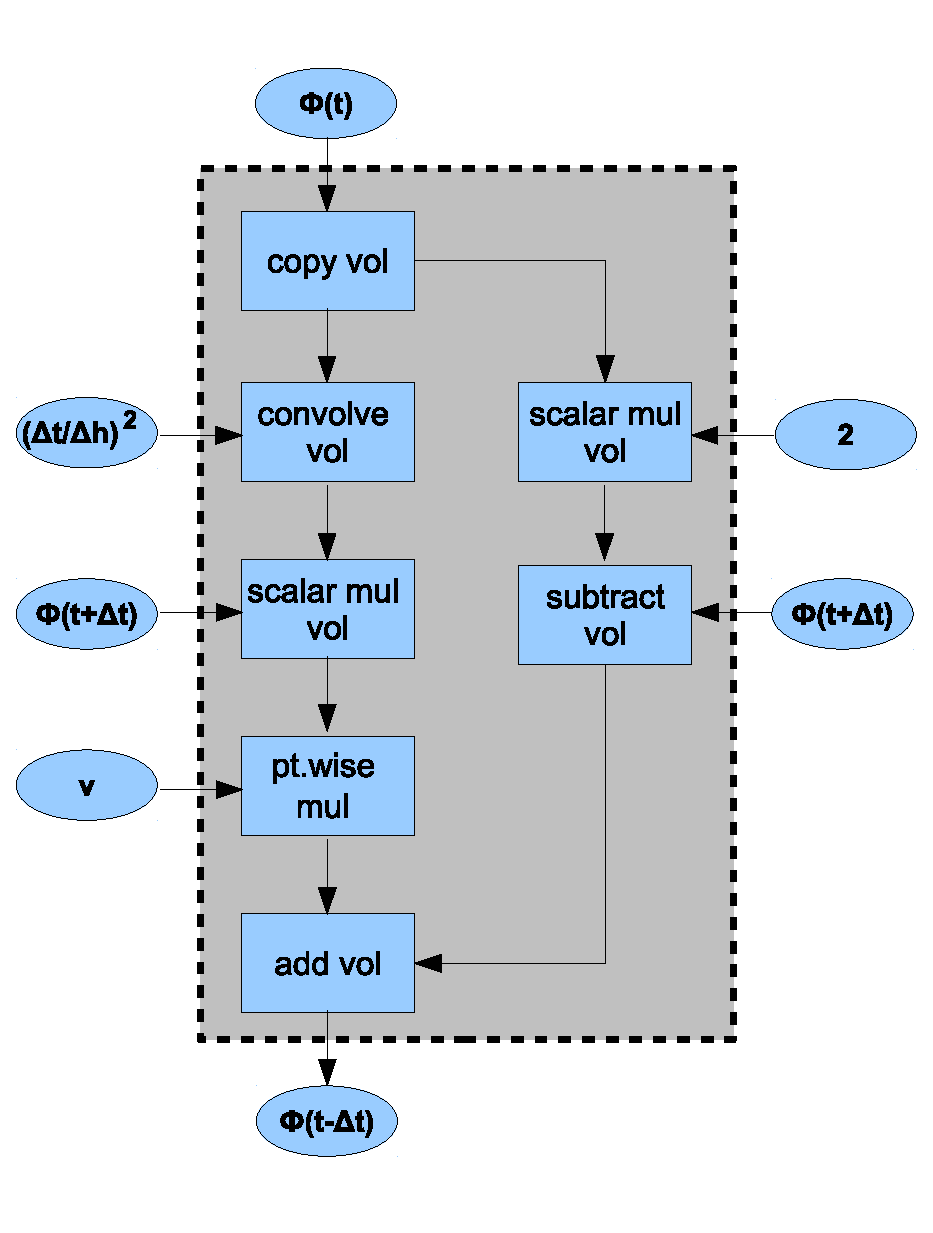
\includegraphics[width = 0.6\linewidth]{./SWE_Update.eps}
\end{center}
\vspace{-1.3cm}
\caption{Implementation of a single update step in the backward time evolution of the scalar
wave equation in accordance with \eqnref{eqn:BTE_SWE}.\label{fig:SWE_Update}}
\end{figure}

All of the migration algorithms are based  
on the solution of the wave equation in one or the other way.  
The scalar wave equation describing the propagation of the 
sound wave in the subsurface is given by
\begin{equation}
\partial_t^2 \, \Phi = v^2\,\Delta\,\Phi\,.
\end{equation}
Here $\Phi=\Phi(t,x,y,z)$ represents the scalar sound wave as a function of space and time and
$v=v(x,y,z)$ is the speed of sound as a function of the subsurface position. In order to simulate
the propagation on a computer, space time has to be discretized on a four dimensional lattice. 
The discretized version of the second order derivative in the 
temporal direction is given by 
\begin{equation}
\partial_t^2\,\Phi = \frac{\Phi(t+\Delta t)-2\,\Phi(t)+\Phi(t-\Delta t)}{\Delta t^2} + \mathcal{O}(\Delta t^2)\,.
\end{equation}
Here $\Delta t$ is the lattice spacing along the temporal direction.
The laplacian $\Delta^2$ can be represented in a similar way by a stencil 
operator $\tilde{\Delta}^2$ on the lattice. 
If we imply the same lattice spacing along the spatial directions, i.e. $\Delta x = \Delta y = \Delta z \equiv \Delta h$, it is given by
\begin{eqnarray}
\Delta h^2\,\Delta \Phi(t,x,y,z)& = & \phantom{+} \Phi(t,x+\Delta h,y,z) + \Phi(t,x-\Delta h,y,z) \nonumber\\
				&   & + \Phi(t,x,y+\Delta h,z) + \Phi(t,x,y-\Delta h,z) \nonumber\\
				&   & + \Phi(t,x,y,z+\Delta h) + \Phi(t,x,y,z-\Delta h) \nonumber\\
				&   & - 6\,\Phi(t,x,y,z)+\mathcal{O}(\Delta h^4) \nonumber\\
                                & = & \phantom{+}\tilde{\Delta} \Phi(t,x,y,z)+\mathcal{O}(\Delta h^4)\,.
\end{eqnarray}
This can be written as a convolution of the scalar field with a matrix $[\tilde{\Delta}]$
\begin{equation}
\tilde{\Delta} \Phi(t,x,y,z) = \sum_{i,j,k} [\tilde{\Delta}]_{ijk}\, \Phi(t,x+i,y+j,z+k)~~,~~i,j,k\in \{-1,0,1 \}\;
\end{equation}
where the elements of the matrix $[\tilde{\Delta}]$ are given by
\begin{equation}
[\tilde{\Delta}]_{i,j,-1}=[\tilde{\Delta}]_{i,j,1}= \left(
\begin{array}{ccc}
0 & 0 & 0 \\
0 & 1 & 0 \\
0 & 0 & 0 
\end{array}
\right) ~~,~~
[\tilde{\Delta}]_{i,j,0}= \left(
\begin{array}{ccc}
0 & 1  & 0 \\
1 & -6 & 1 \\
0 & 1  & 0 
\end{array}
\right)~.
\end{equation}
Hence, 
the backward evolution of the scalar wave field on the lattice is given by
\begin{equation}
\Phi(t-\Delta t) = \hat{v}^2 \,\tilde{\Delta} \Phi(t) + 2\,\Phi(t) - \Phi(t+\Delta t)~~,~~\hat{v}=\frac{\Delta t}{\Delta h}\, v~.\label{eqn:BTE_SWE}
\end{equation}
Here $\hat{v}$ is the dimensionless velocity field. 
This is the equation which we want to implement. In the presented framework,
the scalar field is nothing but a volume object and the velocity field is a velocity 
object as one would expect. 
In order to implement an update step, one needs two volume objects representing the scalar field
at time $t$ ($\Phi(t)$) and at time $t+\Delta t$ ($\Phi(t+\Delta t)$). As an output, one obtains
the distribution of the scalar wave at time $t-\Delta t$.

A possible realisation of \eqnref{eqn:BTE_SWE} in the given framework is shown in \figref{fig:SWE_Update}.
One duplicates the input field $\Phi(t)$ in order to process the given volume in two branches. The branch
on the left hand side corresponds to the application of the discretized laplacian and the multiplication with the 
dimensionless velocity field squared. The branch on the right hand side corresponds to the scalar multiplication of $\Phi(t)$ by a factor of two and the subsequent subtraction with $\Phi(t+\Delta t)$. At the end, one adds the 
two branches in order to obtain the final result. 
 

\end{document}